% !TEX root = ../notes.tex

\section{The Fundamental Group}

\subsection{Circles and Stuff}
We are going to talk about circles and loops and use these to talk about the ideas of groups.
\begin{figure}[!ht]
  \centering
  \begin{tikzpicture}
    \begin{knot}[
        % draft mode=crossings ,
        clip width=3,
        flip crossing=1,
        flip crossing=2,
        ]
        \strand [ultra thick] (0,0) circle (1.0cm);
        \strand [ultra thick] (1,0) circle (1.0cm);
    \end{knot}
  \end{tikzpicture}
\end{figure}
Then we can define something known as a loop,
\begin{ndefi}[Loop]
  An oriented curve that has the same start and end point.
\end{ndefi}
Loops with the same start point can be glued together to create one loop and we can state the following,
\begin{nlemma}[]
  If we take two loops curling about a circle, then denote the number of turns as $B_m$ and $B_n$ and then as we connect these loops, we can say we have the curve $B_{m+n}$.
\end{nlemma}
The proof of this is simple and obvious. We can do a similar thing with Borromean rings.

\begin{figure}[!ht]
\centering
\begin{tikzpicture}
\begin{knot}[
    %draft mode=crossings ,
    clip width=4,
    ]
    \strand [ultra thick] (0,0) circle (1.0cm);
    \strand [ultra thick] (1,0) circle (1.0cm);
    \strand [ultra thick] (0.5,1) circle (1.0cm);
    \flipcrossings{1, 2, 5, 6}
\end{knot}
\end{tikzpicture}
\end{figure}
and pull the third ring into a $U$ shape between the other two rings. We can then talk about a group, where going through the circle $A$, one way is $a$, the other being $b^{-1}$. Similarly, we can talk about $b$ and $b^{-1}$. Hence, the Borromean rings have a loop of $aba^{-1}b^{-1}$. Moving onwards towards the fundamental group, we can say this,
\begin{intu}
  The fundamental group of a space $X$ will be defined so that its elements are loops in $X$ starting and ending at a point $x_0 \in X$.
\end{intu}
Loops in the fundamental group are unique up to deformations.


\subsection{Basic Constructions}
We are going to define some stuff, firstly paths,
\begin{ndefi}[Path]
  A path in a space $X$ we are talking about $f : I \to X$
\end{ndefi}
and now we formalise a homotopy,
\begin{ndefi}[Homotopy of paths]
  A homotopy of paths in $X$ is a family $f_t : I \to X$ for some $t \in [0,\,1]$ and such that,
  \begin{itemize}
    \item $f_t(0) = x_0$ and $f_t(1) = x_1$, the endpoints of the curve are independent of $t$.
    \item The associated map $F : I \times I \to X$ is defined by $F(s, t) = f_t(s)$.
  \end{itemize}
  When we can say that $f_0$ and $f_1$ are connected by a homotopy $f_t$, they are said to be homotopic, notated by $f_0 \hm f_1$.
\end{ndefi}

Now we can define some sort of equivalence on them in the following proposition,
\begin{nprop}
  The relation of homotopy on paths with fixed endpoints in any space is an equivalence relation.
\end{nprop}
\begin{proof}
  We need to prove the following three things,
  \begin{itemize}
    \item \textbf{Reflexivity: }This is evident, where we just take $f = f_t$.
    \item \textbf{Symmetry: }This is also evident, we just take the inverse homotopy, i.e. $f_{1-t}$.
    \item \textbf{Transitivity: }For transitivity, we construct a homotopy from $f_0$ to $f_1$, then $g_0$ and $g_1$. We then define them as, $H(s, t) =F(s, 2t)$ for $t \in \left[0,\,\frac{1}{2}\right]$ and $H(s, t) = G(s, 2t-1)$ for $t \in \left[\frac{1}{2},\,1\right]$. It's continuous on the whole as it's continuous on it's parts.
  \end{itemize}
\end{proof}

From this proof we can define a product paths,
\begin{ndefi}[Product Paths]
  If we have two paths, $f, g : I \to X$ such that $f(1) = g(0)$, there is a \textbf{composition} or \textbf{product path} $f \cdot g$ that traverses first $f$, then $g$, defined by,
  $$ \begin{cases}
    f(s) & s \in \left[0 ,\, \frac{1}{2}\right]\\
    g(2s-1) & s \in \left[\frac{1}{2},\, 1\right]
  \end{cases} $$
\end{ndefi}

\begin{ndefi}[Fundemental Group]
  We define the Fundemental group as the set of all homotopy classes $[f]$ for loops, $f: I \to X$ at the basepoint $x_0$. Denoted $\pi_1(X, x_0)$
\end{ndefi}

Now, we don't really know if this a group yet, so let's prove it.
\begin{nprop}
  $\pi_1(X, x_0)$ is a group with respect to the product, $[f][g] = [f \cdot g]$
\end{nprop}
\begin{proof}
  We just have to prove the three axioms of the group, as we know that $[f][g] = [f \cdot g]$ is well defined. We are going to consider a reparameterisation of our maps, through a $\phi : I \to I$ where $\phi(0) = 0$ and $\phi(1)=1$, this preserves the homotopy class as $f\phi \hm f$ and finally define the homotopy of $\phi$, just to be the linear homotopy.
  \begin{itemize}
    \item \textbf{Inverse: }We let the inverse loop, just be the loop where we replace $t \mapsto 1 - t$
    \item \textbf{Identity: }We just let the identity be the constant map.
    \item \textbf{Associativity: }This is basically taking three loops and then just joining them, so you go across every loop, just at different speeds.
  \end{itemize}
\end{proof}

If we take some $h : I \to X$ and let it be a path, then we can consider the fact of whether the following fundamental groups are equivalent, $\pi_1(X, x_0)$ and $\pi_1(X, x_1)$. Luckily, if we let $h$ start at $x_0$ and end at $x_1$, then we can consider for each loop $f$ based at $x_1$ to another loop $h \cdot f \cdot \overline{h}$ which starts at $x_0$, we note that $\overline{h}$ is just the reversal of $h$. Hence, we now define a change of basepoint map,
\begin{ndefi}[Change Of Basepoint]
  A map $\b_h: \pi_1(X, x_1) \to \pi_1(X, x_0)$ by $\b_h[f] = [h \cdot f \cdot \overline{h}]$.
\end{ndefi}
This is well defined because if $f_t$ is a homotopy of loops, then we have an inverse nicely.

\begin{nprop}
  The map $\b_h$ is an isomorphism
\end{nprop}
\begin{proof}
  Notice,
  \begin{align*}
    \b_h[f \cdot g] &= [h \cdot f \cdot g \cdot \overline{h}]\\
    &= [h \cdot f \cdot \ol{h} \cdot h \cdot g \cdot \ol{h}]\\
    &= \b_h[f] \b_{h}[g]
  \end{align*}
  and it has an inverse as,
  \begin{align*}
    \b_{h}\b_{\ol{h}}[f] &= \b_h[\ol{h} \cdot f \cdot h]\\
    &= [h \cdot \ol{h} \cdot f \cdot h \cdot \ol{h}]\\
    &= [f]
  \end{align*}
  and similarly for the other direction.
\end{proof}


\begin{nprop}
  A space $X$ is simply connected iff there is a unique homotopy class of paths connecting any two points in $X$.
\end{nprop}

\begin{proof}
  This proof relies for the forward direction on proving uniqueness of paths, then if $f \hm f \cdot \overline{g} \cdot g \hm g$ and so it's unique. The other direction is if there is only one homotopy class, then all loops will be homotopic to the constant loop and so, $\pi_1(X, x_0) = 0$.
\end{proof}

\subsection{Fundemental Group of the Circle}

We are going to try and prove that $\fg {S^1} \hm \Z$

\begin{nthm}[]
  $\fg {S^1}$ is an infinite cyclic group generated by the homotopy class of the loop $\omega(s) = (\cos 2\pi s, \sin 2\pi s)$ based at $(1, 0)$.
\end{nthm}

Before we do this, we shall talk about some stuff \footnote{A James note to James, I hate this section of the book, it's messy and not very readable.}

\begin{ndefi}[Lift]
  If we take a $p : \R \to S^1$ such that, $p(s) = (\cos 2\pi s, \sin 2\pi s)$ and another, $\wt{\omega} : I \to \R$, that we define as $\wt{\omega}_n (s) = ns$. Then, we call $\wt{\omega}_n$ the \textbf{lift} of $\omega_n$.
\end{ndefi}

and also,
\begin{ndefi}[Covering Space]
  A \textbf{covering space} of a space $X$ consists of a space $\wt{X}$ and a map, $p : \wt{X} \to X$ satisfying the following,
  \begin{itemize}
    \item For each $x \in X$ there is an open neighbourhood $U$ of $x$ such that $p^{-1}(U)$ is a union of disjoint open sets each of which is mapped homeomorphically onto $U$ by $p$.
  \end{itemize}
\end{ndefi}

\begin{ndefi}[Evenly Covered]
  We call such a $U$, as in the previous definition, \textbf{evenly covered}.
\end{ndefi}

Here are three important things that we will need to prove the theorem,
\begin{enumerate}
  \item For each path starting at $x_0\in X$ and each $\wt{x_0} \in p^{-1}(x_0)$ there exists a unique lift $\wt{f} : I \to \wt{X}$ starting at $\wt{x_0}$.
  \item For each homotopy $f_t : I \to X$ of paths starting at $x_0$ and each $\wt{x_0} \in p^{-1}(x_0)$ there is a unique lifted homotopy $\wt{f} : I \to \wt{X}$ of paths starting at $\wt{x_0}$
  \item Given a map $F : Y \times I \to X$ and a map $\wt{F}: Y \times \{0\} \to wt{X}$ lifting $F | Y \times \{0\}$, then there is a unique map $\wt{F} : Y \times I \to \wt{X}$ lifting $F$ and restricting to the given $\wt{F}$ on $Y \times \{0\}$.
\end{enumerate}
I shall not state the proofs, but they are true.

\begin{proof}[\textbf{Proof of Theorem 1.12}]
  To prove this, take a loop with basepoint $(1, 0)$ and let that be an element of $\pi_1(S^1, x_0)$. Then apply $(1)$, then note that $\wt{f}$ starts at $0$ ends at some integer. Then we have another path from $0$ to $n$, $\omega_n$, such that ${f} \hm \omega_n$ so that, $[f] = [\omega_n]$.\\
  Next prove that $n$ is unique, by stating two $\omega$'s and then let them be delimited by $n$ and $m$, then prove that $n = m$ by using $(b)$ and then the uniqueness part of $(a)$.
\end{proof}
Then, finally both, $(a)$ and $(b)$ can be derived from $(c)$. For $(a)$, let $Y$ be a point and for $(b)$ we let $Y = I$.\\

\begin{nthm}[FTA]
  Every nonconstant polynomial with coefficients in $\C$ has roots in $\C$.
\end{nthm}
\begin{proof}
  Take a polynomial ($p(z) = z^n + a_1z^{n-1} + \dots + a_n$) that has no roots in $\C$ and then consider,
  $$ f_r(s) = \frac{p(re^{2\pi is})/p(r)}{|p(re^{2\pi is})/p(r)|} $$
  which is a loop and as you vary $r$, you get a homotopy of loops based at $1$. Hence, $[f_r] \in \fg {S^1}$. Now choose an $r > 1$ and $r > |a_1| + \dots + |a_n|$. Then for $|z| = r$ we have,
  $$ |z^n| > (|a_1| + \dots + |a_n|)|z^{n-1}| > |a_1z^{n-1}| + \dots + |a_n| \ge |a_1z^{n-1} + \dots + a_n| $$
  Now define a $p_t = z^n + t(a_1z^{n-1} + \dots + a_n)$ and then define a lift and then use Theorem 1.12. This gives, $[\omega_n] = [f_r] = 0$ and hence $n = 0$ and so $p(z) = a_0$ and so that is the only polynomial with no roots and so FTA proved.
\end{proof}

\begin{nthm}[Brouwers fixed points in dimension 2]
  Every continuous map $h : D^2 \to D^2$ has a fixed point, that is, a point $x \in D^2$ with $h(x) = x$.
\end{nthm}
\begin{proof}
  We are going to assume that $h(x) \neq x$ for all $x \in D^2$, then we can define a map $r : D^2 \to S^1$ as defined in the figure. It's obvious that $r$ is continuous. To describe $r(x)$ we say, $r(x) = x$ if $x \in S^1$. Thus $r$ is a retraction of $D^2$ onto $S^1$. Now show that this retraction can't exist.\\
  Let $f_0$ be any loop in $S^1$. In $D^2$ there is a homotopy of $f_0$ to a constant loop. Since the retraction $r$ is the identity on $S^1$, then $rf_1$ is a homotopy in $S^1$ from $f_0$ to $x_0$, however we know that $\pi_1(S^1) \ne 0$, hence contradiction is found.
  \begin{figure}[!ht]
  \centering
  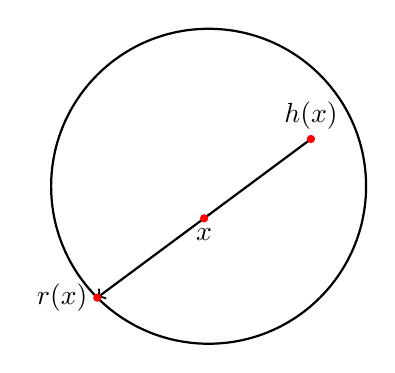
\begin{tikzpicture}
    \draw[thick, ->] (1.3, 0.6) -- (-1.414, -1.414);
    \draw[thick] (0,0) circle (2 cm);
    \fill[fill=red] (1.3,0.6) circle (1.5pt);
    \node[above] at (1.3, 0.6) {$h(x)$};
    \fill[fill=red] (-1.414, -1.414) circle (1.5pt);
    \node[left] at (-1.414, -1.414) {$r(x)$};
    \fill[fill=red] (-0.0571, -0.4071) circle (1.5pt);
    \node[below] at (-0.0571, -0.4071) {$x$};
  \end{tikzpicture}
  \caption{Brouwers in 2D}
  \end{figure}
  \end{proof}

\begin{nthm}[2D Borsuk-Ulam]
  For every continuous map $f : S^2 \to \R^2$ there exists a pair of antipodal points $x$ and $-x$ in $S^2$ with $f(x) = f(-x)$.
\end{nthm}

\begin{ncor}
  Whenever $S^2$ van be represented as the union of three closed sets, then at least one of those sets contain a pair of antipodal points.
\end{ncor}
\begin{proof}
  Consider a measure distance $d_i : S^2 \to \R$ and define it as, $d_i(x) = \inf_{y \in A_i} \left | x - y\right|$. Then apply Borsuk-Ulam and consider cases.
\end{proof}

We choose three as this is the best case, for example consider a sphere inscribed in a tetrahedron. This object doesn't contain a pair of antipodal points. We can prove a similar result for $S^n$ with $n+1$ different sets.

\begin{figure}[!ht]
\centering
\tdplotsetmaincoords{60}{111}
\begin{tikzpicture}[tdplot_main_coords]
 \coordinate (O) at (0,0,0);
% S^2
\draw[tdplot_screen_coords] (0,0,0) circle (3);
\path (xyz spherical cs:radius=3,latitude=90,longitude=00)
 node[fill,circle,inner sep=2pt]{};
\foreach \X in {0,1,2}
{\draw plot[variable=\t,domain=90:90-109.5,smooth]
 (xyz spherical cs:radius=3,latitude=\t,longitude=\X*120)
 node[fill,circle,inner sep=2pt]{};}
\draw plot[variable=\t,domain=0:360,smooth]
(xyz spherical cs:radius=3,latitude={90-109.5-14*abs(sin(1.5*\t))},longitude=\t);
\end{tikzpicture}
\caption{A sphere split into four}
\end{figure}

We can now say some more about our fundemental group,
\begin{nprop}
  $\fg {X \times Y} \cong \fg X \times \fg Y$ if $X$ and $Y$ are both path connected
\end{nprop}
\begin{proof}
  Use the fact that $f : Z \to X\times Y$ is path connected if and only if $g : Z \to X$ and $h : Z \to Y$ are continuous when $f$ is defined as $f(z) = (g(z),\, h(z))$. We now say that a loop $f$ in $X \times Y$ is equivalent to a pair of loops $g$ and $h$ in $X$ and $Y$ respectively, similarly with homotopies. Thus we get a bijection. Then we see $[f] \mapsto ([g],\, [h])$.
\end{proof}

\begin{eg}[Torus]
  We can define a torus as $S^1 \times S^1$ and now using our new proposition, we can talk about,
  $$ \fg {S^1 \times S^1} \cong \fg {S^1} \times \fg {S^1} \cong \Z \times \Z  $$
  Hence, we can nicely talk about a point $(p, q) \in \Z^2$ as $p$ times around one $S^1$ factor and $q$ times around the other $S^1$ factor. If we take $(3, 2)$, we get the trefoil knot.
  \begin{figure}[!ht]
  \centering
  \begin{tikzpicture}
  \begin{knot}[
    consider self intersections=true,
  %  draft mode=crossings,
    flip crossing=2,
    only when rendering/.style={
  %    show curve controls
    }
    ]
  \strand (0,1) .. controls +(1.1,0) and +(120:-1.1) .. (210:1) .. controls +(120:1.1) and +(60:1.1) .. (-30:1) .. controls +(60:-1.1) and +(-1.1,0) .. (0,1);
  \end{knot}
  \end{tikzpicture}
  \end{figure}
\end{eg}

\subsection{Induced Homomorpisms}
We can consider our $\phi : X \to Y$ where $\phi : \fg {X, x_0} \to \fg {Y, y_0}$ and it takes the basepoint $x_0$ to $y_0$. Then we can say that $\phi_{*} : \fg{X, x_0} \to \fg{Y, y_0}$ defined by composing loops $f : I \to X$ based at $x_0$ with $\phi$, so $\phi_{*}[f] = [\phi f]$. The induced homomorphism $\phi_{*}$ is well-defined since a homotopy $f_t$ of loops based at $x_0$ yields a homotopy of loops $\phi f_t$ based at $y_0$. So,
$$ \phi_{*}[f_0] = [\phi f_0] = [\phi f_1] = \phi_{*}[f_1] $$
We can also say $\phi_{*}$ is a homomorphism as,
$$ \phi (f \centerdot g) = (\phi f) \cs (\phi g) $$
as we can consider $\phi f(2s)$ for $0 \le s \le \frac{1}{2}$ and $\phi g (2s - 1)$ for $\frac{1}{2} \le s \le 1$.
\begin{ndefi}[Induced homomorphisms]
  Two basic properties of induced homomorphisms are,
  \begin{itemize}
    \item $(\psi \phi)_{*} = \psi_* \phi_*$ for a composition $\begin{tikzcd}
    	{(X, x_0)} & {(Y, y_0)} & {(Z, z_0)}
    	\arrow["\psi", from=1-1, to=1-2]
    	\arrow["\phi", from=1-2, to=1-3]
    \end{tikzcd}$.
    \item $\1_* = \1$ i.e. the identity map, $\1 : X \to X$ induces the identity map $\1 : \fg {X, x_0} \to \fg {X, x_0}$
  \end{itemize}
  Note that these two things make the fundemental group a functor\footnote{CATEGORY THEORY TIME}
\end{ndefi}

\begin{nprop}
  $\pi_1 (S^n) = 0$ for $n \ge 2$
\end{nprop}

To prove this, we will need the following,

\begin{nprop}
  If a space $X$ is the union of a collection of path-connected open sets $A_\a$ each containing the basepoint $x_0 \in X$ and if each intersection $A_\a \cap A_\b$ is a path-connected, then every loop in $X$ at $x_0$ is homotopic to a product of loops each of which is contained in a single $A_\a$.
\end{nprop}

\begin{proof}
  Take a loop at a basepoint $x_0$ and then a partition $0 = s_0 < s_1 < s_2 < \dots < s_m = 1$ of $I$ such that each subinterval $[s_{i-1},\, s_i]$ is mapped to a single $A_\a$. \\
  Now denote $A_i$ as $f([s_{i-1},\, s_i])$ and $f_i$ by restricting $f$ to $[s_{i-1},\, s_i]$. Then, as we have path connected sets, we can take a path from $x_0$ to $f(s_i) \in A_{i} \cap A_{i+1}$ and hence consider,
  $$ (f_1 \cs \ol{g_1}) \cs (g_1 \cs f_2 \cs \ol{g_2}) \cs (g_2 \cs f_3 \cs \ol{g_3}) \cs \dots \cs (g_{m-1} \cs {f_{m}}) $$
  and it's homotopic to $f$! Finally this loop is just the composition of a load of loops in each of the subsets.
\end{proof}

\begin{proof}[{Proof of Prop 1.22}]
  We can take $S^n$ and express it as two open sets $A_1$ and $A_2$ (each homeomorphic to $\R^n$), such that $A_1 \cap A_2$ is homeomorphic to $S^{n-1} \times \R$. Choose a basepoint $x_0 \in A_1 \cap A_2$. If $n \ge 2$ then $A_1 \cap A_2$ is path connected. Hence, $\pi_1 {A_1} = \pi_1 {A_2} = 0$. Hence, every loop in $S^n$ is nullhomotopic.
\end{proof}

\begin{ncor}
  $\R^2$ is not homeomorphic to $\R^n$ for $n \ne 2$
\end{ncor}
\begin{proof}
  Suppose we have a homeomorphism and then for $n=1$, it's trivial. Then, for $n>2$ we consider the fundemental groups and then it is trivial for everything but $n=2$.
\end{proof}

\begin{nprop}
  If a space $X$ retracts onto a space $A$, then the homeomorphism induced by the inclusion map, $i : A \emd X$ is injective. If $A$ is a deformation retract, then $i_*$ is a isomorphism.
\end{nprop}

\begin{proof}
  If $r : X \to A$ is a retraction, then $ri = r_*i_* = \1$, which implies that $i_*$ is injective. If $r_t : X \to X$ is a deformation retraction, then we can say that there is a loop such that $r_t f$ gives a homotopy, so $i_*$ is also surjective.
\end{proof}

\begin{ndefi}[Basepoint-preserving homotopy]
  We have a $\phi_t : (X, x_0) \to (Y, y_0)$ such that it is the case that $\phi_t (x_0) = y_0$ for all $t$.
\end{ndefi}

\begin{pprop}[Induced homomorphism]
  We can now talk about another basic property of induced homomorphisms,
  \begin{itemize}
    \item If $\phi_t : (X, x_0) \to (Y, y_0)$ is a basepoint-preserving homotopy, then $\phi_{0*} = \phi_{1*}$
  \end{itemize}
\end{pprop}

Now, at this point, we are really rather annoyed with all this basepoint nonsense, hence we look to drop this condition,

\begin{nprop}
  If $\phi : X\to Y$ is a homotopy equivilence, then the induced homeomorphism $\phi_* : \fg { X, x_0} \to \fg {Y, \phi (x_0)}$ is an isomorphism for all $x_0 \in X$.
\end{nprop}
To prove this, we will prove the following,
\begin{nlemma}[]
  If $\phi_t : X \to Y$ is a homotopy and $h$ is the path $\phi_t(x_0)$ formed by the images of a basepoint $x_0\in X$, then the three maps in the diagram below satisfy $\phi_{0*} = \b_h \phi_{1*}$
\end{nlemma}

\[\begin{tikzcd}
	&& {\pi_1 (Y, \phi_1(x_0))} \\
	{\pi_1 (X, x_0)} \\
	&& {\pi_1 (Y, \phi_0(x_0))}
	\arrow["{\phi_{1*}}", from=2-1, to=1-3]
	\arrow["{\phi_{0*}}"', from=2-1, to=3-3]
	\arrow["{\beta_h}", from=1-3, to=3-3]
\end{tikzcd}\]

\section{Van Kampen's Theorem}
This theorem will allow us to calculate more fundemental groups by just decomposing spaces into smaller spaces and reconstituting those fundemental group. \\

\noindent
If we take the example of two circles at a point we will get something in terms of a free product, namely $\Z * \Z$.

\subsection{Free Products on Groups}
To work out why on earth we want anything like this, let us consider a collection of groups. We want to get one singular group where each of these groups are subgroups. There are obviously two ways we know how to do this,
\begin{itemize}
  \item The product group, $\prod_\a G_\a$, whose elements are regarded as functions $\a \mapsto G_\a$.
  \item The direct sum, $\bigoplus_\a G_\a$, by restricting these functions, taking the non-identities finitely often.
\end{itemize}
The problem comes as then all the elements will commute, we don't want this to happen and so we will construct a nonalbelian version of $\bigoplus_\a G_\a$ called the $*_\a G_\a$.

\begin{ndefi}[Free Product]
  As a set, three product $*_\a G_\a$ consists of all words $g_1g_2g_3\dots g_m$ of arbitrary finite length $m \ge 0$, where each letter $g_i$ belongs to a group $G_{\a_i}$, and is not identity, and adjacent letters $g_i$ and $g_{i+1}$ belong to different groups $G_\a$, that is $\a_i \ne \a_{i+1}$. Words satisfying this are called \textit{reduced}. The empty word is the identity.\\
  The group identity is juxtaposition $(g_1\dots g_m)(h_1\dots h_n) = g_1\dots g_mh_1\dots h_n$.
\end{ndefi}
\begin{remark}
   You can reduce a word by rewriting adjacent letters that lie in the same $G_{\a_i}$ to a single letter and cancel trivial letters.
\end{remark}

We can nicely find that this group is associative.
\begin{proof}
  Let $W$ be thr set of all the reduced words $g_1\dots g_m$ including the empty word. To each $g \in G_\a$ we associate a function $L_g (g_1\dots g_m) = gg_1\dots g_m$ and we combine with $g_1 \in G_\a$ such that it's a reduced word. We can say, $L_{gg'} = L_gL_{g'}$ and this is a special case of associativity, $g(g'(g_1\dots g_m)) = (gg')(g_1\dots g_m)$. We can also say that $L_g$ is invertible with inverse $L_{g^{-1}}$. Hence it's a group homomorphism from $G_\a$ to $P(W)$, the permutations of $W$. More generally we can define $L : W \to P(W)$ by $L(g_1,\dots, g_m) = L_{g_1}\dots L_{g_m}$ for each reduced words $g_1\dots g_m$. The product operation in $W$ corresponds under $L$ to composition in $P(W)$, because of the relation $L_{gg'} = L_gL_{g'}$. Since the composition in $P(W)$ is associative, we conclude that the product in $W$ is associative.
\end{proof}

We can now say something nice about $\Z * \Z$, it's a free product but also a free group! We have some lingo to do with this, we can say that each element is uniquely representable as as reduced words in powers of generators for various copies of $\Z$, one generator for each $\Z$.
\begin{ndefi}[Basis]
  The basis of a free group is all of the generators
\end{ndefi}
\begin{ndefi}[Rank]
  The rank of the free group is just the number of generators.
\end{ndefi}
The abelianization of the free group is a free abelian group with basis of the same set of generators, and so the rank of the abelianization of a group is well defined, independent of choice of basis, the same is true for the rank of the free group.

\begin{nlemma}
  Any two different ways to reduce the word will then produce the same reduced word.
\end{nlemma}
\begin{proof}
  Associativity
\end{proof}

Any collection of homomorphisms $\phi_\a : G_\a \to H$ extends uniquely to $\phi : *_\a G_\a \to H$. Namely, the value of $\phi$ on a word $g_1\dots g_m$ with $g_i \in G_{\a_i}$ must be $\phi_{\a_1}(g_1)\dots \phi_{\a_n}(g_n)$, and using this formula to derive $\phi$ gives a well defined homomorphism since the process of reducing an unreduced product doesn't change it's image.

\subsection{The van Kampen Theorem}
We will take a space $X$ that can be decomposed as the union of a collection of path-connected open subsets $A_\a$. Then, we define $i_{\a\b} : \fg{A_\a \cap A_\b} \to \fg{A_\a}$ as an induced homomorphism by the inclusion $A_\a \cap A_\b \emd A_\a$. Then basically we can get that the kernel of some map $\phi : *_\a \fg{A_\a} \to \fg{X}$ contains all the elements of the form, $i_{\a\b}(\omega)i_{\b\a}(\omega)^{-1}$.

\begin{nthm}[Van Kampen Theorem]
  If $X$ is the union of path-connected open sets $A_\a$ each containing the basepoint $x_0\in X$ and if each intersection $A_\a \cap A_\b$ is path-connected, then the kernel of $\phi$ is the normal subgroup $N$ generated by all elements of the form $i_{\a\b}(\omega)i_{\b\a}(\omega)^{-1}$ for $\omega \in \fg{A_\a \cap A_\b}$, and hence $\phi$ induces an isomorphism $\fg{X} \approx *_\a\fg{A_\a}\setminus N$.
\end{nthm}


\begin{eg}
  We shall consider some $\bigvee_\a S^1_\a$ and van Kampens Theorem states that $\fg{\bigvee_\a S^1_\a}$ is free and so, free product of copies of $\Z$. Hence, $\fg{S^1 \v S^1} = \Z * \Z$. More generally, the fundemental group of any connected graph is free.
\end{eg}

\begin{ndefi}[Normal Subgroup]
   A subgroup $N$ of the group $G$ is normal in $G$ if and only if $gng^{-1} \in N$ for all $g \in G$ and $n \in N$ We denote this as, $N \triangleleft G$.
\end{ndefi}

\begin{proof}[Proof of Van Kampens Theorem]
  We have already proved surjectivity of $\phi$ in Proposition 1.23. Now we prove that $\ker\phi = N$. We shall define the following,
  \begin{ndefi}[Factorisation]
    A factorisation of an element $[f] \in\fg{X}$ we mean a formal product $[f_1]\dots[f_k]$ where,
    \begin{itemize}
      \item Each $f_i$ is a loop in some $A_\a$ at the basepoint $x_0$, and $[f_i]\in \fg{A_\a}$ is the homotopy class of $f_i$.
      \item The loop is homotopic to $f_1, \dots, f_k$ in $X$.
    \end{itemize}
  \end{ndefi}
  \noindent
  A factorisation of $[f]$ is thus a word in $*_\a \fg{A_\a}$, possibly unreduced, that is mapped to $[f]$ by $\phi$. So surjectivity of $\phi$ is equivalent to every word of $[f] \in \fg{X}$ has a factorisation. \\

  \noindent
  \begin{ndefi}[Equivalent Factorisation]
    We shall call two factorisations equivalent if they are related by a sequence of the following moves,
    \begin{enumerate}
      \item Combine adjacent terms $[f_i][f_{i+1}]$ into a single term $[f_i \cs f_{i+1}]$ if $[f_i]$ and $[f_{i+1}]$ are both in the same group $\fg{A_\a}$.
      \item Regard the term $[f_i] \in \fg{A_\a}$ as lying in the group $\fg{A_\b}$ rather than $\fg{A_\a}$ if $f_i$ is a loop in $A_\a \cap A_\b$.
    \end{enumerate}
  \end{ndefi}
  The first move doesn't change the element, and the second doesnt change the image of the element in the quotient group $Q = *_\a\fg{A_\a}\sm N$. We now aim to show that any two factorisations are equivalent, which means $\phi$ is injective, so $\ker \phi = N$.\\
  If we take two factorisations and form a homotopy ($F: I \times I \to X$), we can then form a partition and now what we have is a covering of $I \times I$ with finitely many rectangles ($R_r$'s). Now we do something odd and shift the middle row around such that each point is in at most three rectangles. We can assume that there are at least three rows of these rectangles. We shall index them from the bottom from left to right on each row.\\
  If we take a $\g$ on $I \times I$, from the left side to the right, we can consider $F | \g$, which is then a loop at the basepoint $x_0$ as $F$ maps both the left edge and the right edge to $x_0$. We now consider a path $\g_r$ as the path that separates off the first $r$ rectangles, so $\g_0$ is the bottom edge and $\g_{mn}$ the top.\\
  Now let vertices, $v$, be any corner such that $F(v) \ne 0$. Then, we can choose paths $g_v$ from $x_0$ to $F(v)$ that lie in the intersection of two or three $A_{ij}$'s (image of $R_{r}$ in $F$). Then we obtain a factorisation of $[F | \g_r]$, different choices of which $A_{ij}$ we go into can change our factorisation, however these factorisations are equivalent. Furthermore $\g_r$ and $\g_{r+1}$ are equivalent as we are just pushing through another rectangle.\\
  Finally, we make our $\g_0$ equivalent to our first factorisation by choosing vertices that are on the bottom edge and also not lying in the $A_\a$ such that $v$ is in the domain of $f_i$. We then do something similar for $\g_{mn}$ by letting it be the second factorisation and then we also know that all $\g_r$'s are equivalent and so the factorisations are equivalent.
\end{proof}

Here is an interesting example that I have stewed over since it's been a while since I've picked this up.
\begin{eg}
  \textbf{Torus Knots}: Consider two positive integers that are relatively prime, $m$ and $n$. The torus knot $K = K_{m,\,n} \subset \R^3$ is the image of the embedding $f : S^1 \to S^1 \times S^1 \subset \R^3$, $f(z) = (z^m,\,z^n)$. This is the interesting bit to me, the knot $K$ winds arounds the torus a total of $m$ times in the longitudinal direction and $n$ in the meridional direction. We need to assume that $m$ and $n$ are relatively prime in order for $f$ to be injective otherwise $f$ would be $\gcd(m,\,n)$-to-one, the image of this $f$ would be $K_{\frac{m}{d},\,\frac{n}{d}}$ where $d = \gcd(m,\,n)$. We could also allow negative $m$ and $n$ and that would just change $K$ to be a mirror-image knot.\\
  % knot diagram here
  Let us compute $\fg{\R^3 - K}$, it is easier to compute this fundamental group with $\R^3$ replaced with it's compactification $S^3$. Van Kampens Theorem tells us that this doesn't affect anything and this makes sense. Namely, we are taking the union of $\R^3 - K$ and an open ball $B$ formed by the compactification point together with the complement a large closed ball in $\R^3$ containing $K$. As we used Van Kampens Theorem we require $B$ and $B\cap (\R^3 - K)$ to be simply connected and we find that they are. Hence, $\R^3 - K \emd S^3 - K$ induces an isomorphism on $\pi_1$.\\
  To compute the fundamental group we show that it deformation retracts to a 2D complex $X = X_{m,\,n}$ homeomorphic to the quotient space of a cylinder $S \times I$ under the identifications $(z,\,0) \sim (e^{\frac{2\pi i}{m}}z,\,0)$ and $(z,\,1) \sim (e^{\frac{2\pi i}{n}}z,\,1)$. We define $X_m$ and $X_n$ as the left and right halves of $X$.\\
  If we consider $\fg{X}$, then we can decompose this into the union of the fundemental groups of $X_m$ and $X_n$. Both $X_m$ and $X_n$ deformation retract onto circles and so they fundemental group of (open balls around) $X_m$ and $X_n$ are just $\Z$, we also note that $X_m \cap X_n$ is also a circle and so the $\fg(X_m \cap X_n) = \Z$. If we consider a loop in $X_m \cap X_n$ that is a generator is homotopic in $X_m$ to $m$ times a generator and in $X_n$ it's homotopic to $n$ times a generator. VKT then tells that $\fg(X)$ is now just the quotient of the free group on generators $a$ and $b$ obtained by factoring out the normal subgroup generated by $a^mb^{-n}$. \\

  We denote $G_{m,\,n}$ this group generated by $a$ and $b$ and with one relation $a^m = b^n$. If $m = 1$ or $n = 1$ then $G$ is just infinite cyclic then one generator is a power of another. To find the behaviour, let us consider the center of this group. We can see that $a^m = b^n$ commutes with $a$ and $b$ and so the cyclic group $C$ is generated by $a^m = b^n$. Moreover, $C$ is normal, so we can consider $G \sm C$, which is just the free product $\Z_m * \Z_n$. The free product of non-trivial groups has a trvial center, hence $C$ is the center of $G$. Finally we can show that $m$ and $n$ are uniquely determined by $\Z_m * \Z_n$.
\end{eg}

\subsection{Application of Cell Complexes}
Take some $2$-cells $e^2_\a$ and attach them to a path-connected space $X$ via some map, $\varphi : S^1 \to X$ (as we defined in the introduction) to produce a new space, $Y$. If $s_0$ is a basepoint of $S^1$, we shall call $\varphi_\a(s_0)$ a loop even though it isn't of the usual form. Now we get a loop from $x_0 \in X$, a basepoint, and a path $\g_\a$ from $x_0$ to $\varphi_\a(s_0)$ and now we have the basic setup for the next proposition.

\begin{nprop}
  The following three hold,
  \begin{enumerate}
    \item If $Y$ is obtained from $X$ by attaching $2$-cells as described above, then the inclusion $X \emd Y$ induces a surjection $\pi_1(X, x_0) \to \pi_1 (Y, x_0)$ whose kernel is the normal subgroup generated by all the loops $\g_\a\varphi_\a\overline{\g_\a}$, $N$. Thus, $\fg Y \cong \fg X / N$
    \item If $Y$ is obtained from $X$ by attaching $n$-cells for a fixed $n > 2$, then the inclusion $X \emd Y$ induces an isomorphism $\pi_1(X, x_0) \cong \pi_1(Y, x_0)$
    \item For a path connected cell complex $X$ the inclusion of the $2$-skeleton $X^2 \emd X$ induces an isomorphism $\pi_1(X^2, x_0) \cong \pi_1(Y, x_0)$
  \end{enumerate}
\end{nprop}

\begin{proof}
  The proof of (i) relies on considering a slightly larger space. Consider the path between $x_0$ and each of the $e_\a^2$ cells, then we extrude these upwards and call them $S_\a$. Now we call this space $Z$. $Z$ deformation retracts onto $Y$. Now we consider two different situations, take $Z$ and puncture each of the $2$-cells anywhere by where they intersect $S_\a$, then we can say this space deformation retracts to $X$, call it $A$. Now consider $Z - X$, then this will contract to a point and so it is contractible, call this space $B$. Since $\fg B = 0$, then an application of Van Kampens Theorem tells us that $\fg Z \cong \fg A / N$ where $N$ is the image of $\fg {A \cap B} \to \fg A$ \\

  \noindent
  For (ii), we can use a similar if not identical argument but with $e_\a^n$ cells instead of $e^2_\a$ and so we get the $\fg {S^{n-1}} = 0, (n > 2)$ as we proved earlier.\\

  \noindent
  For (iii), we prove by induction for the finite case. For the non-finite case we argue as such, we aim to take a loop $f: I \to X$ that has a basepoint $x_0 \in X^2$. Then as aim to prove that $\pi_1(X^2, x_0) \to \pi_1(X, x_0)$ is bijective. The surjection comes from the fact $f$ has a compact image in $X^n$ and so $f$ is homotopic to some loop in $X^2$. For the injection suppose we have some $g$ that is nullhomotopic in $X^2$, then again it's compact and we apply (b) to get the injection and so we can conclude that $f$ is also nullhomotopic in $X^2$.
\end{proof}

\noindent
Now we consider an orientable surface, which is $0$-cell, $2g$ $1$-cells and a $2$-cell. We can then talk about the fundamental group of this object we know a $1$-skeleton is just the wedge sum of $2g$ circles and it has a fundamental group that's free on two generators. Then we know the $2$- cell is just the product of the commutators of the generators and so,
$$ \fg {M_g} = \braket{a_1, b_1, \dots, a_g, b_g}{[a_1, b_1] \dots [a_g, b_g]} $$
This is some new notation,
\begin{notation}
   We write $\braket{g_\a}{r_\b}$ to mean a group with generators $g_\a$ and relators $r_\b$. In other words, $\pi_1(M_g) = \gen{g_\a} / \gen{r_\b}$.
\end{notation}

Now here a fun little result,
\begin{ncor}
   The surface $M_g$ is not homeomorphic, or even homotopy equivalent to $M_h$ if $g \ne h$.
\end{ncor}

\subsubsection{Commutator}
Here's also some more slightly interesting background mathematics that we need for the proof. We call the commutator of two elements $g$ and $h$, $[g, h] = g^{-1}h^{-1}gh$; however we also may say that $[g, h] = ghg^{-1}h^{-1}$. This commutator is equal to $e$ if and only if $gh = hg$. Here are a couple of facts,
\begin{enumerate}
  \item $[g, h]^{-1} = [h, g]$
  \item $[g, h]^s = [g^s, h^s]$ where $g^s = sgs^{-1}$, the conjugate of $g$ by $s$.
  \item For any homomorphism, $f : G \to H$, we can say $f([g, h]) = [f(g), f(h)]$.
\end{enumerate}
Note that the third implies the second as it's a generalisation, it tells us that the set of conjugators is stable under some $f : G \to G$ (where we take $G = H$). These also show us that the set of commutators is closed under inversion and conjugation. Which takes us to a new definition,
\begin{ndefi}[Commutator Subgroup]
  Take the set of commutators, $G'$, of a group, by the identities above, then $G'$ is a subgroup of $G$.
\end{ndefi}

\noindent
Furthermore, $([g_1, h_1][g_2, h_2]\dots [g_n, h_n])^s = [g_1^s, h_1^s][g_2^s, h_2^s] \dots [g_n^s, h_n^s]$ and so we can say $G'$ is a normal subgroup.

\begin{ndefi}[Abelianisation]
  Consider a group $G$ and it commutator subgroup $G'$, then the abelianisation of $G$ is $G / G'$ and is denoted $G^{\text{ab}}$.
\end{ndefi}

\noindent
We can do some category theory and see that the map $\varphi : G \to G^{\text{ab}}$ is universal.

\begin{proof}
  The abelianisation of $\fg {M_g}$ is the direct sum of $2g$ copies of $\Z$. Hence if, $M_g \hm M_h$, then $\fg {M_g} \cong \fg {M_h}$. Hence the abelianisations are isomorphic and so $g = h$.
\end{proof}

For non-orientable surfaces we can do something similar. Consider $g$ circles and we attach a $2$-cell by the word $a_1^2a_2^2a_3^2\dots a_n^2$ we then get a non-orientable surface, $N_g$. For some examples $N_1$ is just $\R \mathrm{P}^2$ (for babies) and $N_2$ just a klein bottle. We can say that $\fg {N_g} = \braket{a_1, \dots, a_n}{a_1^2\dots a_n^2}$ and so the abelianisation of this is the direct sum of $\Z_2$ with $g$ copies of $\Z$ as we can choose the generators such that $2(a_1 + \dots + a_n) = 0$.
Hence $N_g \not\hm N_h$ if $g \ne h$ or even $N_g \not\hm M_h$ for any surfaces. \\

\noindent
Here is something else,
\begin{ncor}
   For every group $G$ there is a $2$-dimensional cell complex $X_G$ with $\fg{X_G} \cong G$.
\end{ncor}
\begin{proof}
  Choose a representation of $G = \braket{g_\a}{r_\b}$ as every group is the quotient of some free group. Then let $g_\a$ be the generators of the free group and $r_\b$ be the generators of the kernel of the map from the free group to the group. Now let $X_G$ be constructed from $\bigvee_\a S^1_\a$ by attaching the loops of $r_\b$ (which are $2$-cells) .
\end{proof}